\documentclass[12pt]{article}
\usepackage{mathpazo}
\usepackage{hyperref}
\usepackage{amsmath}
\usepackage{enumitem}
\usepackage{graphicx}
\usepackage{xcolor}
\usepackage{textcomp}
\usepackage{booktabs}
\usepackage{longtable}
\usepackage{soul}
\setuldepth{model}
\usepackage{everysel}

% This is to fix full justification for \texttt{}. Credit:
% https://texblog.net/latex-archive/plaintex/full-justification-with-typewriter-font/
\ttfamily
\fontdimen2\font=0.4em% interword space
\fontdimen3\font=0.2em% interword stretch
\fontdimen4\font=0.1em% interword shrink
\fontdimen7\font=0.1em% extra space

% Credit: Stefan Kottwitz, https://latex.org/forum/viewtopic.php?t=13230
\newcommand*{\Biggg}[1]{\vcenter{\hbox{\scalebox{3}{\ensuremath#1}}}}
\newcommand*{\Bigggg}[1]{\vcenter{\hbox{\scalebox{8}{\ensuremath#1}}}}

\usepackage[top=2.54cm, bottom=2.54cm, left=2.54cm, right=2.54cm]{geometry}
\usepackage{tikz}
\usetikzlibrary{fit}
\usetikzlibrary{calc}
\usetikzlibrary{matrix}
\usetikzlibrary{calligraphy}
\usetikzlibrary{arrows.meta}
\usetikzlibrary{shapes.misc}
\usetikzlibrary{intersections}
\usetikzlibrary{shapes,arrows}
\usetikzlibrary{shapes.multipart}
\usetikzlibrary{shapes.geometric}
\usetikzlibrary{shadows,shadings}
\usetikzlibrary{tikzmark,positioning}
\usetikzlibrary{decorations.markings}
\usetikzlibrary{decorations.pathreplacing}

\tikzstyle{stochnode}=[black, draw=black, line width=1.5pt, shape=circle, fill=white, minimum size=8mm, inner sep=3pt]

\tikzstyle{detnode}=[black, draw=black, line width=1.5pt, densely dashed, shape=circle, fill=white, minimum size=8mm, inner sep=3pt]

\tikzstyle{constnode}=[black, draw=black, line width=1.5pt, shape=regular polygon, regular polygon sides=4, fill=white, minimum size=8mm, inner sep=1pt, align=center]

\tikzstyle{clampnode}=[black, draw=black, line width=1.5pt, shape=circle, fill=black!20!white, minimum size=8mm, inner sep=3pt]

\begin{document}
\frenchspacing

\begin{center}
{\Large \textbf{Lab 7. Bayesian inference using RevBayes, continued}} \\[0.5cm]
{\large Due Sunday, November 20, 2022 at 3 pm}
\end{center}

\vspace{1cm}

\noindent In today's lab, we are going to pick up where we left off last week and continue our RevBayes journey. First, we will use Rev -- the language underlying RevBayes -- to write our own simple Markov chain Monte Carlo (MCMC) simulation, in order to get a sense of what exactly it is doing and why it works. Next, we will apply our knowledge of Rev and MCMC to phylogenetics, and learn about some challenges that are specific to Bayesian phylogenetic inference: namely, prior choice. \\

\hrule

\section*{Part 1: Archery and Markov chain Monte Carlo}

\begin{center}
\textcolor{blue}{What follows has been adapted from a RevBayes tutorial developed by Prof. Tracy Heath's lab at the Iowa State University. You can access the full version from \\
\url{https://revbayes.github.io/tutorials/mcmc/archery.html}}
\end{center}

\noindent Last time, we mentioned that most of the time, we cannot calculate posterior distributions analytically, that is, with pen and paper. Instead, we have to rely on simulations. The idea of estimating parameter values using simulation is surprisingly old and long predates the existence of electronic computers (look up \textit{Buffon's needle} if you are interested), but it wasn't until sufficiently powerful computers became available in the 1990s that one such simulation method, called ``Markov chain Monte Carlo'' or MCMC for short, exploded in popularity. \\

\noindent To make sure we understand what MCMC is doing, we will once again start with a simple, tractable model. Specifically, we will estimate the probability distribution of an archer's arrows landing at a particular distance from the center of a target:

\begin{center}
\noindent\includegraphics[width=0.4\textwidth]{archery.png}
\end{center}

\noindent To construct our model, we will assume that these distances follow an exponential distribution with some unknown mean $\mu$ (mu), which corresponds to the \textit{expected distance} from the bullseye. We could interpret this as an estimate of the archer's skill: an experienced archer's $\mu$ would be smaller than a beginner's. The exponential distribution tells us that an arrow is much more likely to land at a small distance from the center than at a large distance:

\begin{center}
\noindent\includegraphics[width=0.8\textwidth]{target_accuracy.pdf}
\end{center}

\noindent Let's further assume our Bayesian archer shot $n$ arrows at the target, with some average distance $\bar{d}$ from the bullseye. It turns out that $\bar{d}$ follows a gamma distribution with two parameters: the shape, here equal to $n$, and the rate, equal to $\frac{n}{\mu}$. (We've already encountered the gamma distribution in Lecture 10.3, when modeling rate variation across characters.) The mean $m$ of the gamma distribution can be computed as:

\[ m = \frac{\text{shape}}{\text{rate}} = \frac{\,n\,}{\frac{n}{\mu}} = \mu \]

\noindent We already know this quantity: it represents the expected distance \textit{from the bullseye}, or the archer's \textit{accuracy}. The variance $v$ of our gamma distribution is equal to 

\[ v = \frac{\text{shape}}{\text{rate}^2} = \frac{n}{\left(\frac{n}{\mu}\right)^2} = \frac{\mu^2}{n} \]

\noindent and represents the archer's \textit{precision}, or dispersion: how far the arrows are expected to land \textit{from each other}.

\noindent If we recall what we learned last week, we can immediately tell that our gamma distribution represents a model with two parameters, $n$ and $\mu$. Of these, the number of arrows $n$ is known and fixed, while the expected distance $\mu$ is a free parameter that we are going to estimate. To do so, we first need to place a prior distribution on it. In this example, we are going to use an exponential prior distribution, with a single parameter denoted $\lambda$ (lambda). We are going to set $\lambda$ to 1, but we could also imagine making this parameter larger (if we had strong reason to believe that the archer is very accurate) or smaller (if we believed the opposite). \\

\noindent Returning to the graphical notation introduced in our previous lab, we can represent this model as follows:

\begin{figure}[h]
\centering
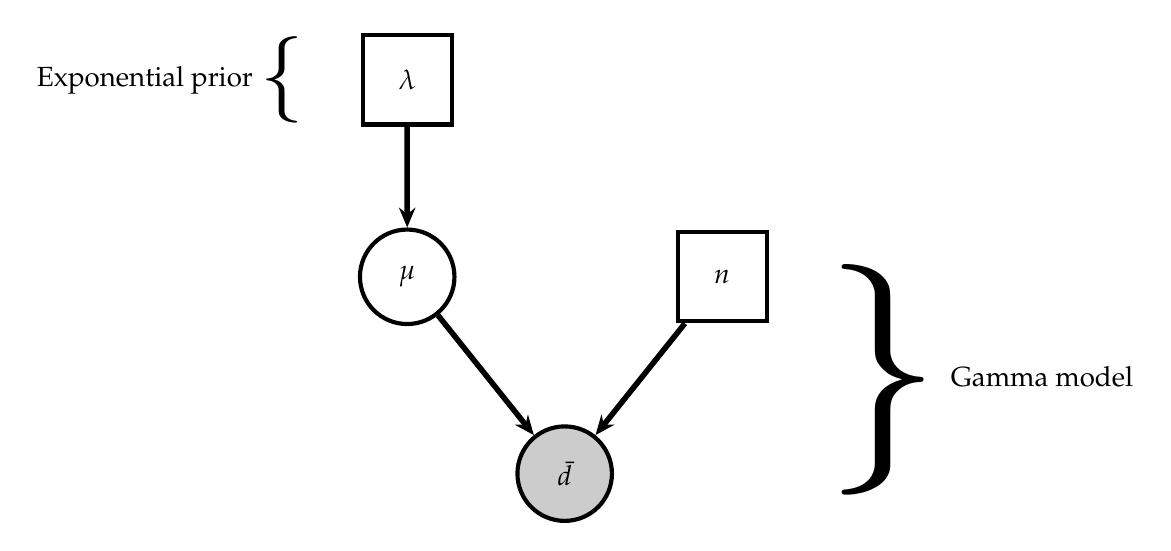
\begin{tikzpicture}
\node [constnode, minimum size=16mm] (lambda) at (0,2) {$\lambda$};
\node [stochnode, minimum size=12mm] (mu) at (0,-0.5) {$\mu$};
\node [constnode, minimum size=16mm] (n) at (4,-0.5) {$n$};
\node [clampnode, minimum size=12mm] (dbar) at (2,-3) {$\bar{d}$};
\node (unif) at (-3,2) {Exponential prior $\Biggg\{$};
\node (binom) at (7.25,-1.8) {$\Bigggg\}$ Gamma model};

\draw[-{Stealth[length=0.25cm, width=0.25cm, angle'=45]}, line width=2pt, color=black] (lambda) -- (mu);
\draw[-{Stealth[length=0.25cm, width=0.25cm, angle'=45]}, line width=2pt, color=black] (mu) -- (dbar);
\draw[-{Stealth[length=0.25cm, width=0.25cm, angle'=45]}, line width=2pt, color=black] (n) -- (dbar);
\end{tikzpicture}
\end{figure}

\noindent The last thing we are going to need before we start the inference process is some actual data $\bar{d}$. It turns out that RevBayes can be of assistance in this case, too: we are going to cheat and generate our data using the very model we just created, based on some pre-defined ``true'' value of $\mu$. I use the word ``cheat'' in a very facetious manner here, because this workflow is actually perfectly valid and very convenient. In particular, it allows us to directly compare the estimated value of $\mu$ to its known true value, which we can't ever do with real data. (If we knew the true values of our parameters, all inference would clearly be superfluous.) With this in mind, let's get started! \\

\noindent Note that the different assignment operators we learned about last time tell RevBayes how different variables should be treated within its own MCMC machinery. Today, however, we are building our own MCMC simulator from scratch, so we can stick with the constant-variable assignment operator, \texttt{<-}: \\

\indent \texttt{lambda <- 1.0} \\
\indent \texttt{n <- 10}

\newpage

\noindent Our ``true'' $\mu$ value, \texttt{mu\_true}, can be whatever we want it to be: \\

\indent \texttt{mu\_true <- 1.0} \\

\noindent Finally, using the \texttt{rgamma()} function, I'm going to make one draw (first argument) from a gamma distribution with a shape of \texttt{n} (second argument) and a rate of \texttt{n/mu\_true} (third argument): \\

\indent \texttt{arrow\_mean <- rgamma(1, n, n/mu\_true)[1]} \\

\noindent Our first step is to initialize the MCMC simulation with some starting value for the estimated parameter $mu$, which we will do by storing a draw from our exponential prior in yet another constant variable: \\

\indent \texttt{mu <- rexp(1, lambda)[1]} \\

\noindent Next, let's do something new: define our own function describing the likelihood of $\mu$. This function will take a proposed value of $\mu$ as its input, and return its probability density conditional on the observed data as its output. Once again, the syntax is similar to \textsf{R}: the \texttt{function} keyword is used to define a function, and the \texttt{return} keyword is used to return the output. Below, we tell RevBayes to treat the likelihood as gamma-distributed if the proposed value is non-negative, and to set it to 0 if the proposed value is negative: \\

\indent \texttt{function likelihood(mu) \{} \\
\indent \texttt{\ \ \ \ if (mu < 0.0) \{} \\
\indent \texttt{\ \ \ \ \ \ \ \ return 0.0} \\
\indent \texttt{\ \ \ \ \} else \{} \\
\indent \texttt{\ \ \ \ \ \ \ \ return dgamma(arrow\_mean, n, n/mu, log=false)} \\
\indent \texttt{\ \ \ \ \}} \\
\indent \texttt{\}} \\

\noindent We can define another function to describe the prior probability of a proposed $\mu$ value. Note that in agreement with our definition of prior probabilities, this function does not depend on the data (\texttt{arrow\_mean}): \\

\indent \texttt{function prior(mu) \{} \\
\indent \texttt{\ \ \ \ if (mu < 0.0) \{} \\
\indent \texttt{\ \ \ \ \ \ \ \ return 0.0} \\
\indent \texttt{\ \ \ \ \} else \{} \\
\indent \texttt{\ \ \ \ \ \ \ \ return dexp(mu, lambda, log=false)} \\
\indent \texttt{\ \ \ \ \}} \\
\indent \texttt{\}} \\

\newpage

\noindent We can also prepare a log file in which we will store the sampled values of $\mu$: \\

\indent \texttt{\# The file is going to have two columns, called "iteration" and "mu"} \\
\indent \texttt{write("iteration", "mu", "\textbackslash n", file="archery.log")} \\
\indent \texttt{\# Write down the initial value of mu, which we have drawn above} \\
\indent \texttt{write(0, mu, "\textbackslash n", file="archery.log", append=TRUE)} \\

\noindent And let's print them to the screen as well: \\

\indent \texttt{print("iteration", "mu")} \\
\indent \texttt{print(0, mu)} \\

\noindent Now that all the ingredients are in place, let's take a detailed look at what our MCMC simulator is going to do:

\begin{enumerate}
  \item Generate an initial value for $\mu$ -- \textbf{done!}
  \item Based on the current value $\mu$, draw a new value (denoted $\mu'$, or ``mu prime'') from some proposal distribution $q$
  \item Calculate the acceptance ratio $R$ as follows:
  
  \begin{align*}
  R &= \min\left\{1, \, \frac{p(\bar{d} \, | \, \mu')}{p(\bar{d} \, | \, \mu)} \times \frac{p(\mu')}{p(\mu)} \times \frac{q(\mu)}{q(\mu')} \right\} \\[1ex]
      &= \min\left\{1, \, \text{likelihood ratio} \times \text{prior ratio} \times \text{proposal ratio} \right\}
  \end{align*}
  
  Note that we read $\min\left\{\right\}$ as ``the smaller of''. Therefore, either the product of the three ratios turns out to be greater than 1, in which case we are always going to accept the newly proposed value $\mu'$ (= accept with a probability of 1), or it turns out to be smaller, in which case we will only accept $\mu'$ with probability $R$. What does that mean, you ask? That's where our next step comes in:
  \item Draw a random (uniformly distributed) number $u$ from 0 to 1. \\[1ex]
  \textbf{if} $\boldsymbol{u <}$ \textbf{R:} \\
  \hspace*{20pt} Accept the proposal and set $\mu = \mu'$ \\
  \textbf{else:} \\
  \hspace*{20pt} Reject the proposal and keep $\mu$ at its current value.
  \item Record the current value
  \item Go back to step 2
\end{enumerate}

\newpage

\noindent All that remains to do is to translate this into Rev. We will use a fixed number of iterations (20,000), storing the sampled parameter values every 20 iterations. We will also use a uniform proposal distribution $q$. As we will see in a moment, this distribution will be centered on the current value of $\mu$, meaning that the difference between the upper bound of the distribution and $\mu$ will be the same as the difference between $\mu$ and the lower bound of the distribution. We will call this difference \texttt{delta} and set it equal to 1: \\

\indent \texttt{n\_iter = 20000} \\
\indent \texttt{printgen = 20} \\
\indent \texttt{delta = 1} \\

\noindent This \texttt{delta} would be an example of what we call a \textit{tuning parameter} in MCMC terminology, because it tunes the behavior of our proposal. Making it very small ensures that the newly proposed value $\mu'$ will be very close to the current value $\mu$. This will make it very likely to get accepted, but it will make the exploration of different values slow and difficult. Conversely, making it very large will favor bold jumps far away from the current value, many of which will, however, end up in regions of low posterior probability and get rejected. Modern MCMC implementations are often capable of ``auto-tuning'' (yes, really) their proposals. \\

\noindent Since we want to repeat the same series of operations many times, the natural construct to use is a \texttt{for} loop: \\

\indent \texttt{for(iter in 1:n\_iter) \{} \\
\indent \texttt{\ \ \ \ \# Step 2: propose a new value of mu} \\
\indent \texttt{\ \ \ \ mu\_prime <- mu + runif(n=1, -delta, delta)[1]} \\

\noindent This is our Rev implementation of the uniform proposal distribution described above. We draw a number ranging from negative \texttt{delta} to positive \texttt{delta} (here, from $-1$ to 1), and add it to the current value of $\mu$ to generate a new, proposed value $\mu'$. \\

\noindent Next, we will use the functions we defined above to compute the prior probabilities and likelihoods of the proposed and current values, which we will in turn use to compute the acceptance ratio $R$: \\

\indent \texttt{\ \ \ \ \# Step 3: compute the acceptance probability} \\
\indent \texttt{\ \ \ \ R <- likelihood(mu\_prime)/likelihood(mu) * prior(mu\_prime)/prior(mu)} \\

\noindent What happened to the third term of the product, the proposal ratio? It turns out that for the uniform proposal distribution we chose to use, it is always going to be equal to 1, so we can just leave it out and move on: \\

\indent \texttt{\ \ \ \ \# Step 4: accept or reject the proposal} \\
\indent \texttt{\ \ \ \ u <- runif(1 ,0, 1)[1] } \\

\newpage

\indent \texttt{\ \ \ \ if (u < R) \{} \\
\indent \texttt{\ \ \ \ \ \ \ \ \# Accept the proposal} \\
\indent \texttt{\ \ \ \ \ \ \ \ mu <- mu\_prime} \\ 
\indent \texttt{\ \ \ \ \}} \\

\noindent Finally, we will store the current value of $\mu$ to our log file and print it to the screen. To ensure that we only do this every 20th iteration like we said we would, we will divide the current iteration number (\texttt{iter}) by our \texttt{printgen} variable, and only proceed if the remainder is equal to 0: \\

\indent \texttt{\ \ \ \ \# Step 5: record the current value} \\
\indent \texttt{\ \ \ \ if ( (iter \% printgen) == 0 ) \{} \\
\indent \texttt{\ \ \ \ \ \ \ \ \# Write the sampled value to a file} \\
\indent \texttt{\ \ \ \ \ \ \ \ write(iter, mu, "\textbackslash n", file="archery.log", append=TRUE)} \\
\indent \texttt{\ \ \ \ \ \ \ \ \# Print the sampled value to the screen} \\
\indent \texttt{\ \ \ \ \ \ \ \ print(iter, mu)} \\
\indent \texttt{\ \ \ \ \}} \\

\noindent End the MCMC simulation by closing the entire \texttt{for} loop with a matching right curly brace: \\

\indent \texttt{\}} \\

\noindent Hit Enter / Return to execute. We're done!

\vspace*{1ex}

\begin{center}
\textcolor{red}{For your convenience, all of the above code has been packaged into a single Rev script available from Canvas (\texttt{archery.Rev}). You can execute a script in RevBayes as follows:} \\
\textcolor{red}{\texttt{source("/path/to/script.Rev")}}
\end{center}

\vspace*{1ex}

\hrule
\ \\[1ex]
\textbf{1) Open your log file in Tracer. What is the posterior mean of $\mu$? How close is it to the true value?} \\

\noindent \textbf{2) Repeat the analysis with \texttt{mu\_true} set to 0.25, but \texttt{lambda} still set to 1. How did this affect the results? Recall our lectures on Bayesian inference. Why do you think the posterior distribution changed? Is the result ``wrong'' in light of your prior beliefs?} \\

\noindent \textbf{3) In RevBayes, the uniform proposal distribution has been pre-implemented for us as \texttt{mvSlide}, which also accepts the \texttt{delta} tuning argument. Refer to the previous lab (and to the online version of this tutorial, if you like) and re-write our archery exercise in such a way that it makes use of the standard RevBayes machinery (clamped stochastic variables, moves, monitors, the \texttt{mcmc()} function). Submit your answer as a Rev script, i.e., a plain-text file with the \texttt{.Rev} file extension that stores all of your commands.} \\
\hrule

\newpage

\section*{Part 2: Bayesian phylogenetics}

We are now familiar enough with RevBayes to try our hand at the task for which it was designed: Bayesian phylogenetic inference.

\vspace*{1ex}

\begin{center}
\textcolor{blue}{What follows has been adapted from RevBayes tutorials developed by April M. Wright (Southeastern Louisiana University), Michael J. Landis (Washington University in St. Louis), Sebastian H\"{o}hna (Ludwig-Maximilians-Universit\"{a}t), Tracy A. Heath (Iowa State University), and Brian R. Moore (University of California, Davis). You can access the full versions from 
\url{https://revbayes.github.io/tutorials/morph_tree/} and \url{https://revbayes.github.io/tutorials/ctmc/}.}
\end{center}

\vspace*{1ex}

\noindent First, we will load a character matrix into our RevBayes workspace. RevBayes is fine with Nexus files, but wants them to be clean. We will therefore delete the \texttt{ASSUMPTIONS} block (that is, the last four lines) from our \texttt{Tedford\_2009-1.nex} file. We will assign the contents of our dataset to a new workspace object called \texttt{morpho}: \\

\indent \texttt{morpho = readDiscreteCharacterData("/Users/David/Tedford\_2009-1.nex")} \\

\noindent We can immediately create a few ``helper'' variables that will come in handy later on. From the \texttt{mopho} object, we can extract the number of taxa in our analysis (here, 39) and plug it into the formula for the number of branches in our unrooted tree ($2n - 3$). This will tell us how many branch lengths we will have to estimate. We can also get a list of taxon names, which we will use to initialize our tree: \\

\indent \texttt{num\_taxa <- morpho.size() } \\
\indent \texttt{num\_branches := 2 * num\_taxa - 3} \\
\indent \texttt{taxa <- morpho.names()} \\

\noindent Just like in Lab 6, we will create two more workspace variables to hold our moves and monitors: \\

\indent \texttt{moves = VectorMoves()} \\
\indent \texttt{monitors = VectorMonitors()} \\

\noindent We can also specify our outgroup right away: \\

\indent \texttt{out\_group <- clade("Hesperocyoninae")} \\

\noindent Now we are ready to place a prior probability distribution on the topology of our tree, which is the main parameter we are interested in. We will assume that all $(2n - 5)!!$ unrooted topologies for $n$ taxa have equal probability, that is, we will specify a \textit{uniform} distribution over topologies: \\

\indent \texttt{topology {\footnotesize $\sim$} dnUniformTopology(taxa, outgroup=out\_group)} \\

\noindent We see that \texttt{topology} is a stochastic variable drawn from the specified prior distribution. To estimate it, we need to place some \textit{moves} or \textit{proposals} on it. As it turns out, the topology moves we use in Bayesian phylogenetic inference are no different from those we used for our maximum-parsimony and maximum-likelihood analyses, which we learned about in Lecture 5.4. Here, we will use the nearest-neighbor interchange (NNI) and subtree prune-and-regraft (SPR) moves. As you may recall, SPR is a bit more sophisticated than NNI, so we may want to use it more sparingly: say, one SPR move per every ten NNI moves. We can do this by specifying \textit{weights} for our moves, which tell RevBayes how often they should be applied per iteration, or relative to other moves: \\

\indent \texttt{moves.append( mvNNI(topology, weight=num\_branches) )} \\
\indent \texttt{moves.append( mvSPR(topology, weight=num\_branches/10.0) )} \\

\noindent From our maximum-likelihood lectures, we know that the probability of a character going from one state to another depends not just on the topology of our tree, but also on its branch lengths. As a result, we have to estimate these as well, and since we are working in the Bayesian framework, if we want to estimate them, we first have to place a prior probability distribution on them. As we'll see further down below, choosing the right prior distribution for branch lengths can be tricky. For now, we are just going to use a uniform distribution from 0 to 5, which indicates that all values from 0 to 5 expected changes per character are equally likely: \\

\indent \texttt{for (i in 1:num\_branches) \{} \\
\indent \texttt{\ \ \ \ branch\_lengths[i] {\footnotesize $\sim$} dnUniform(0, 5)} \\
\indent \texttt{\ \ \ \ moves.append( mvScale(branch\_lengths[i]) )} \\
\indent \texttt{\}} \\

\noindent In the loop above, we draw our branch lengths one by one from the specified prior, and add them to a newly created vector called \texttt{branch\_lengths}. With each new branch length, we also define a move that will propose new values for it, and append it to the previously created \texttt{moves} vector. \\

\noindent Up until now, we have recorded the values of each parameter we estimated. With branch lengths, however, there is a problem: they only have a meaning when associated with a particular topology. Between the two of them, RevBayes and Tracer will try to tell you that, for example, \texttt{branch\_lengths[26]} (the 26th element of your branch length vector) has a posterior mean of 0.05, but because the 26th branch of one topology can be associated with a completely different clade than the 26th branch of another topology, that doesn't mean anything much in particular. However, one quantity that we can meaningfully compare across different topologies is tree length, or the sum of all branch lengths: \\

\indent \texttt{tree\_length := sum(branch\_lengths)} \\

\noindent Note that we defined \texttt{tree\_length} as a deterministic variable: it can vary, so it can't be constant, but its value is fully determined by the individual branch lengths -- it cannot vary independently of them. \\

\noindent Similarly, a phylogram -- which is what we are estimating here -- is fully determined by its topology and branch lengths. We will therefore assemble it from the topology and branch lengths we've already specified. Specifically, using the \texttt{treeAssembly()} function, we will tell RevBayes to apply the $i$-th element of the \texttt{branch\_lengths} vector to the branch subtending the $i$-th node in \texttt{topology}, and store the result in another deterministic variable: \\

\indent \texttt{tree := treeAssembly(topology, branch\_lengths)}

\begin{flushright}
\fbox{\begin{minipage}{16.52cm}
\textbf{An alternative approach} \\

\noindent Often, there is more than one way to do things in RevBayes. Above, we went through a 3-step process where we first drew from a \textit{distribution of topologies}, then from a \textit{distribution of branch lengths}, and finally assembled a phylogram out of both draws. We could simplify this approach by drawing directly from a \textit{distribution of phylograms}: \\

\hspace*{12pt} \texttt{\small tree {\footnotesize $\sim$} dnUniformTopologyBranchLength(taxa,} \\
\hspace*{12pt} \texttt{\small \ \ \ \ \ \ \ \ \ \ \ \ \ \ \ \ \ \ \ \ \ \ \ \ \ \ \ \ \ \ \ \ \ \,\,\ \ \ \ outgroup=out\_group,} \\
\hspace*{12pt} \texttt{\small \ \ \ \ \ \ \ \ \ \ \ \ \ \ \ \ \ \ \ \ \ \ \ \ \ \ \ \ \ \ \ \ \ \,\,\ \ \ \ branchLengthDistribution=dnUniform(0, 5))} \\

\noindent We can apply the same moves to our phylogram as we did to our topology: \\

\hspace*{12pt} \texttt{moves.append( mvNNI(tree, weight=num\_branches) )} \\
\hspace*{12pt} \texttt{moves.append( mvSPR(tree, weight=num\_branches/10.0) )} \\

\noindent Since we specified our branch lengths all at once instead of one by one (by means of the \texttt{branchLengthDistribution} argument of the \texttt{dnUniformTopologyBranchLength()} function), we also need a move that is capable of operating on all branch lengths at once: \\

\hspace*{12pt} \texttt{moves.append( mvBranchLengthScale(tree, weight=num\_branches) )} \\

\noindent Finally, we can still set up our tree length variable, but we need to do it a bit differently: \\

\hspace*{12pt} \texttt{tree\_length := tree.treeLength()}
\end{minipage}}
\end{flushright}

\vspace*{1.8ex}

\noindent At this point, the only thing we need to add to our overall model is the \textit{substitution model}, which gives us the exact probabilities of going from one state to a different state along a branch of a given length. We'll use the same model we learned about when going over maximum likelihood, i.e., Paul Lewis's M$k$ (Markov $k$-state) model, with the optional addition of ascertainment bias correction (M$k$v) and among-character rate variation (M$k$+$\Gamma$). \\

\noindent Let's start with the latter. You may remember from Lecture 10.3 that we usually assume that the rates of different characters follow a gamma ($\Gamma$) distribution, and that we set its rate $\beta$ equal to its shape $\alpha$, so that the mean $\frac{\alpha}{\beta}$ equals 1. This leaves us with $\alpha$ as the only parameter we need to estimate. We will therefore treat $\alpha$ as a stochastic variable, draw it from some prior distribution, and place a move on it: \\

\indent \texttt{\# Let\textquotesingle s use a broad uniform distribution from 0 to 1,000,000:} \\
\indent \texttt{alpha {\footnotesize $\sim$} dnUniform(0, 1E6)} \\
\indent \texttt{moves.append( mvScale(alpha, weight=2.0) )} \\

\noindent You may also recall that to simplify the calculations, we break up -- or ``discretize'' -- the continuous gamma distribution into a number of rate categories (usually four). This is easy to do in RevBayes: \\

\indent \texttt{\# The three arguments are: (1) shape, (2) rate, (3) number of categories} \\
\indent \texttt{char\_rates := fnDiscretizeGamma(alpha, alpha, 4)} \\

\noindent Just like before, we want to make sure that each character receives a rate matrix of the right dimensions: a binary character should be described by a 2-by-2 matrix, a three-state character by a 3-by-3 matrix, etc. You still remember what a nightmare it was to convince IQ-TREE to do this for us. The good news is that with RevBayes, doing this is a lot easier. As long as we know the maximum number of character states in our matrix, we can iterate over different state numbers (2, 3, 4, etc.), and for each number $i$, we can extract all the $i$-state characters in our matrix and assign them an $i$-by-$i$ rate matrix: \\

\indent \texttt{max\_num\_states <- 6} \\
\ \\
\indent \texttt{\# Define a helper variable to count distinct rate matrices:} \\
\indent \texttt{j = 1} \\
\ \\
\indent \texttt{\# We will start from 2, because there are no constant (1-state) characters} \\
\indent \texttt{\# in the Tedford et al. matrix} \\
\indent \texttt{for (i in 2:max\_num\_states) \{} \\

\noindent We will create temporary copies of our character matrix, which we can freely modify without the original data being affected. Each copy will form one element of a vector called \texttt{partitions}. To make sure that the 2-state partition forms the 1st element, the 3-state partition forms the 2nd element, etc., we will make sure that the index is one smaller than the current number of states: \\

\indent \texttt{\ \ \ \ partitions[i - 1] <- morpho} \\
\indent \texttt{\ \ \ \ } \\
\indent \texttt{\ \ \ \ \# Only keep those characters whose number of states equals i} \\
\indent \texttt{\ \ \ \ partitions[i - 1].setNumStatesPartition(i)}

\newpage

\noindent We could imagine a case in which our dataset contains, say, 2-state, 3-state, and 5-state characters, but no 4-state characters. To prevent our loop from stumbling over such a case, we will check whether the number of $i$-state characters is greater than zero, and only move on if it is: \\

\indent \texttt{\ \ \ \ \# How many i-state characters do we have?} \\
\indent \texttt{\ \ \ \ nc = partitions[i - 1].nchar()}
\indent \texttt{\ \ \ \ } \\
\indent \texttt{\ \ \ \ if (nc > 0) \{} \\
\indent \texttt{\ \ \ \ \ \ \ \ Q[j] := fnJC(i)} \\

\noindent What happened here? We created an M$k$ rate matrix with $k = i$ states. From Paul Lewis's 2001 paper linked in Lab 5, you may remember that the M$k$ model for morphological data was derived by generalizing an earlier Jukes-Cantor (JC) model for DNA sequences. This explains why the function for setting up an M$k$ model is called \texttt{fnJC()} in RevBayes. It takes a single argument corresponding to the desired number of states, and since the M$k$ model has no free parameters, its rate matrix is fully determined by this number, making it a deterministic variable. Once the rate matrix has been created, we assign it to the $j$-th element of a vector called \texttt{Q}. \\

\noindent Next, we are going to put it all together: \\

\indent \texttt{\ \ \ \ \ \ \ \ characters[j] {\footnotesize $\sim$} dnPhyloCTMC(tree=tree, Q=Q[j], type="Standard",} \\
\indent \texttt{\ \ \ \ \ \ \ \ \ \ \ \ \ \ \ \ \ \ \ \ \ \ \ \ \ \ \ \ \ \ \ \ \ \ \ \ \ \ \ \ \ \ \ siteRates=char\_rates,} \\
\indent \texttt{\ \ \ \ \ \ \ \ \ \ \ \ \ \ \ \ \ \ \ \ \ \ \ \ \ \ \ \ \ \ \ \ \ \ \ \ \ \ \ \ \ \ \ coding="variable")}  \\

\noindent A lot has happened here! We built a stochastic variable for the character data by drawing from a distribution called the \textit{phylogenetic continuous-time Markov chain}, or \texttt{dnPhyloCTMC} for short. This distribution ties together everything we've specified so far: the tree topology with branch lengths (jointly specified by \texttt{tree}), the substitution model (specified through its rate matrix \texttt{Q}), and the model of how rates of change vary across characters (\texttt{char\_rates}). We additionally told RevBayes that it would be dealing with morphological (``standard'') data, and asked it to correct for ascertainment bias by specifying that only variable characters should be considered (\texttt{coding="variable"}). \\

\noindent Now we just have to clamp this variable to our observed character data: \\

\indent \texttt{\ \ \ \ \ \ \ \ characters[j].clamp(partitions[i - 1])} \\
\indent \texttt{\ \ \ \ \ \ \ \ } \\
\indent \texttt{\ \ \ \ \ \ \ \ \# Increment counter} \\
\indent \texttt{\ \ \ \ \ \ \ \ j = j + 1} \\
\indent \texttt{\ \ \ \ \ \ \ \ } \\
\indent \texttt{\ \ \ \ \ \ \ \ \# Close the if-conditional and the for-loop} \\
\indent \texttt{\ \ \ \ \}} \\
\indent \texttt{\}} \\

\begin{flushright}
\fbox{\begin{minipage}{16.52cm}
\textbf{Ordered characters} \\

\noindent So far we have assumed that all our multistate characters are unordered, and as such correctly described by the M$k$ model. This happens to be true of the Tedford et al. dataset we are using as an example, but other matrices may contain a mixture of ordered and unordered characters. This is how we would deal with such a situation in RevBayes: \\

{\footnotesize
\hspace*{12pt} \texttt{ordered\_char\_indices <- [14, 23, 32, 38, 41, 57]} \\
\ \\
\hspace*{12pt} \texttt{\# Create temporary copies of the character data} \\
\hspace*{12pt} \texttt{ordered <- morpho} \\
\hspace*{12pt} \texttt{unordered <- morpho} \\
\ \\
\hspace*{12pt} \texttt{\# Drop all characters and put back only those that are ordered} \\
\hspace*{12pt} \texttt{ordered.excludeCharacter(1:morpho.nchar())} \\
\hspace*{12pt} \texttt{ordered.includeCharacter(ordered\_char\_indices)} \\
\ \\
\hspace*{12pt} \texttt{\# Drop the ordered characters but keep the rest} \\
\hspace*{12pt} \texttt{unordered.excludeCharacter(ordered\_char\_indices)} \\
\ \\
\hspace*{12pt} \texttt{idx = 1} \\
\hspace*{12pt} \texttt{ix = 1} \\

\hspace*{12pt} \texttt{\# Only multistate characters can be ordered, so we start iterating from 3} \\
\hspace*{12pt} \texttt{for (i in 3:max\_num\_states) \{} \\
\hspace*{12pt} \texttt{\ \ \ \ ordered\_partitions[i - 2] <- ordered} \\
\hspace*{12pt} \texttt{\ \ \ \ ordered\_partitions[i - 2].setNumStatesPartition(i)} \\
\hspace*{12pt} \texttt{\ \ \ \ nco = ordered\_partitions[i - 2].nchar()} \\
\hspace*{12pt} \texttt{\ \ \ \ if (nco > 0) \{} \\
\hspace*{12pt} \texttt{\ \ \ \ \ \ \ \ Q\_ord[idx] := fnOrderedRateMatrix(i)} \\
\hspace*{12pt} \texttt{\ \ \ \ \ \ \ \ char\_ord[idx] {\footnotesize $\sim$} dnPhyloCTMC(tree=tree, Q=Q\_ord[idx], type="Standard",} \\
\hspace*{12pt} \texttt{\ \ \ \ \ \ \ \ \ \ \ \ \ \ \ \ \ \ \ \ \ \ \ \ \ \ \ \ \ \ \ \ \ \, \ \ siteRates=char\_rates, coding="variable")} \\
\hspace*{12pt} \texttt{\ \ \ \ \ \ \ \ char\_ord[idx].clamp(ordered\_partitions[i - 2])} \\
\hspace*{12pt} \texttt{\ \ \ \ \ \ \ \ idx = idx + 1} \\
\hspace*{12pt} \texttt{\ \ \ \ \}} \\
\hspace*{12pt} \texttt{\}} \\

\hspace*{12pt} \texttt{\# Back to unordered characters, which can be binary: start iterating from 2} \\[-0.5ex]
\hspace*{12pt} \texttt{for (j in 2:max\_num\_states) \{} \\[-0.5ex]
\hspace*{12pt} \texttt{\ \ \ \ unordered\_partitions[j - 1] <- unordered} \\[-0.5ex]
\hspace*{12pt} \texttt{\ \ \ \ unordered\_partitions[j - 1].setNumStatesPartition(j)} \\[-0.5ex]
\hspace*{12pt} \texttt{\ \ \ \ nc = unordered\_partitions[j - 1].nchar()} \\[-0.5ex]
\hspace*{12pt} \texttt{\ \ \ \ if (nc > 0) \{} \\[-0.5ex]
\hspace*{12pt} \texttt{\ \ \ \ \ \ \ \ Q\_unord[ix] := fnJC(j)} \\[-0.5ex]
\hspace*{12pt} \texttt{\ \ \ \ \ \ \ \ char\_unord[ix] {\footnotesize $\sim$} dnPhyloCTMC(tree=tree, Q=Q\_unord[ix], type="Standard",} \\[-0.5ex]
\hspace*{12pt} \texttt{\ \ \ \ \ \ \ \ \ \ \ \ \ \ \ \ \ \ \ \ \ \ \ \ \ \ \ \ \ \ \ \ \ \, \ \ \ siteRates=char\_rates, coding="variable")} \\[-0.5ex]
\hspace*{12pt} \texttt{\ \ \ \ \ \ \ \ char\_unord[ix].clamp(unordered\_partitions[j - 1])} \\[-0.5ex]
\hspace*{12pt} \texttt{\ \ \ \ \ \ \ \ ix = ix + 1} \\[-0.5ex]
\hspace*{12pt} \texttt{\ \ \ \ \}} \\[-0.5ex]
\hspace*{12pt} \texttt{\}}
}
\end{minipage}}
\end{flushright}

\noindent We're done! Now we just combine everything into a single model: \\

\indent \texttt{mymodel = model(tree)} \\ 

\noindent Let's see if we can graph this overall model using the notation we introduced in Lab 6: \\

\begin{figure}[h]
\centering
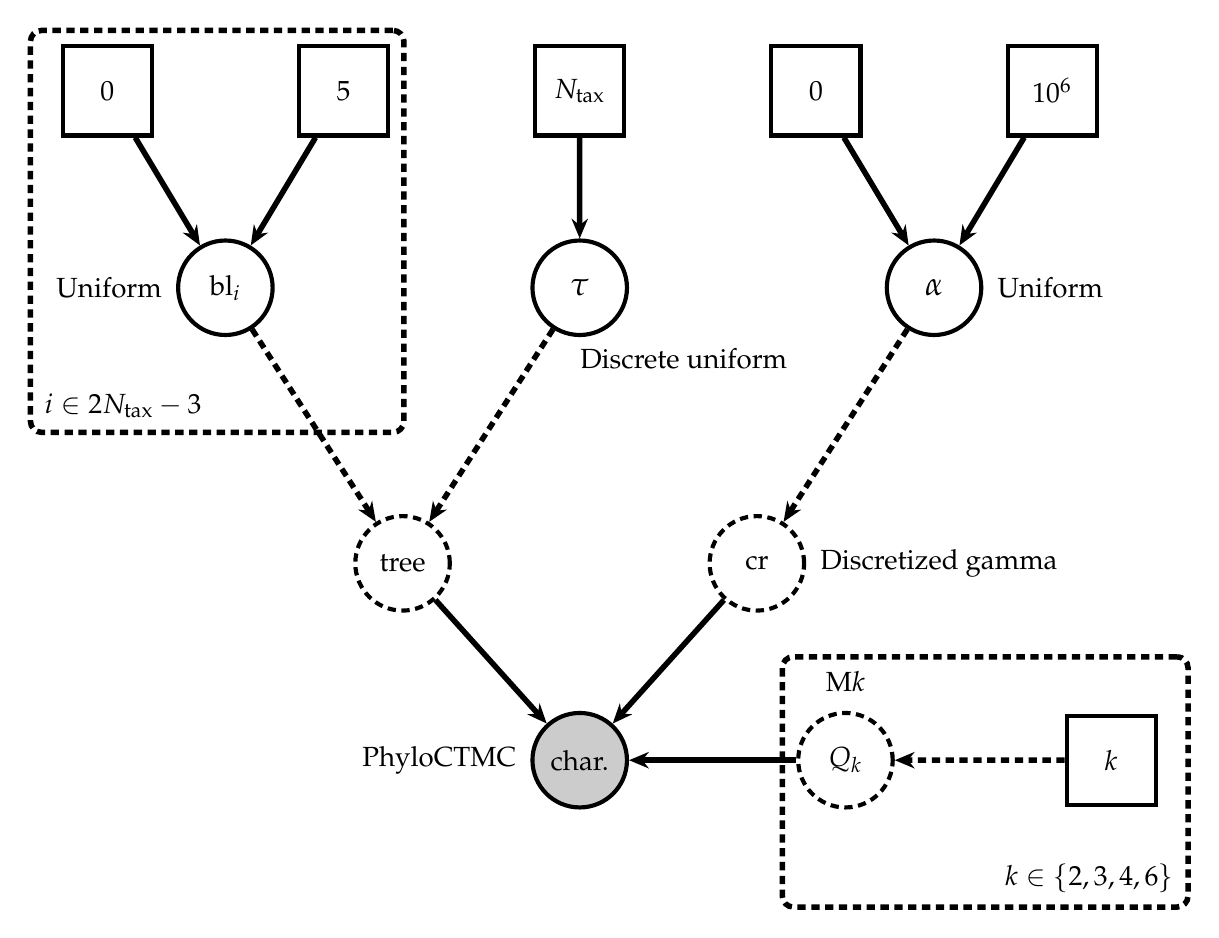
\begin{tikzpicture}
\node [constnode, minimum size=16mm] (unif00) at (0,2) {0};
\node [constnode, minimum size=16mm] (unif01) at (3,2) {5};
\node [constnode, minimum size=16mm] (unif10) at (9,2) {0};
\node [constnode, minimum size=16mm] (unif11) at (12,2) {$10^6$};
\node [constnode, minimum size=16mm] (N) at (6,2) {$N_{\text{tax}}$};
\node [stochnode, minimum size=12mm] (brlen) at (1.5,-0.5) {$\text{bl}_i$};
\node [stochnode, minimum size=12mm] (topology) at (6,-0.5) {\large $\tau$};
\node [stochnode, minimum size=12mm] (alpha) at (10.5,-0.5) {\large $\alpha$};
\node [detnode, minimum size=12mm] (tree) at (3.75,-4) {tree};
\node [detnode, minimum size=12mm] (gamma) at (8.25,-4) {cr};
\node [clampnode, minimum size=12mm] (char) at (6,-6.5) {char.};
\node [constnode, minimum size=16mm] (statenum) at (12.75,-6.5) {$k$};
\node [detnode, minimum size=12mm] (Q) at (9.375,-6.5) {$Q_k$};

\node [shape=rectangle, rounded corners=0mm, inner sep=0pt, anchor=west] (brlennumber) at (-0.8, -2) {$i \in 2N_{\text{tax}} - 3$};
\node [shape=rectangle, rounded corners=0mm, inner sep=0pt, anchor=east] (statenumber) at (13.55, -8) {$k \in \{2, 3, 4, 6\}$};
\node [shape=rectangle, rounded corners=0mm, inner sep=0pt, anchor=east] (distdescr0) at (0.7, -0.5) {Uniform};
\node [shape=rectangle, rounded corners=0mm, inner sep=0pt, anchor=west] (distdescr1) at (6, -1.4) {Discrete uniform};
\node [shape=rectangle, rounded corners=0mm, inner sep=0pt, anchor=west] (distdescr2) at (11.3, -0.5) {Uniform};
\node [shape=rectangle, rounded corners=0mm, inner sep=0pt, anchor=west] (distdescr3) at (9.05, -4) {Discretized gamma};
\node [shape=rectangle, rounded corners=0mm, inner sep=0pt] (distdescr4) at (9.375, -5.5) {M$k$};
\node [shape=rectangle, rounded corners=0mm, inner sep=0pt, anchor=east] (distdescr5) at (5.2, -6.5) {PhyloCTMC};

\node [black, draw=black, line width=2pt, inner sep=5pt, shape=rectangle, rounded corners, densely dashed, fit = (distdescr0) (unif01) (brlennumber)] (brlenplate) {};
\node [black, draw=black, line width=2pt, inner sep=5pt, shape=rectangle, rounded corners, densely dashed, fit = (Q) (distdescr4) (statenumber)] (statenumplate) {};

\draw[-{Stealth[length=0.25cm, width=0.25cm, angle'=45]}, line width=2pt, color=black] (unif00) -- (brlen);
\draw[-{Stealth[length=0.25cm, width=0.25cm, angle'=45]}, line width=2pt, color=black] (unif01) -- (brlen);
\draw[-{Stealth[length=0.25cm, width=0.25cm, angle'=45]}, line width=2pt, color=black] (N) -- (topology);
\draw[-{Stealth[length=0.25cm, width=0.25cm, angle'=45]}, line width=2pt, color=black] (unif10) -- (alpha);
\draw[-{Stealth[length=0.25cm, width=0.25cm, angle'=45]}, line width=2pt, color=black] (unif11) -- (alpha);
\draw[-{Stealth[length=0.25cm, width=0.25cm, angle'=45]}, line width=2pt, densely dashed, color=black] (brlen) -- (tree);
\draw[-{Stealth[length=0.25cm, width=0.25cm, angle'=45]}, line width=2pt, densely dashed, color=black] (topology) -- (tree);
\draw[-{Stealth[length=0.25cm, width=0.25cm, angle'=45]}, line width=2pt, densely dashed, color=black] (alpha) -- (gamma);
\draw[-{Stealth[length=0.25cm, width=0.25cm, angle'=45]}, line width=2pt, densely dashed, color=black] (statenum) -- (Q);
\draw[-{Stealth[length=0.25cm, width=0.25cm, angle'=45]}, line width=2pt, color=black] (tree) -- (char);
\draw[-{Stealth[length=0.25cm, width=0.25cm, angle'=45]}, line width=2pt, color=black] (gamma) -- (char);
\draw[-{Stealth[length=0.25cm, width=0.25cm, angle'=45]}, line width=2pt, color=black] (Q) -- (char);
\end{tikzpicture}
\end{figure}

\noindent Here, $N_{\text{tax}}$ is the number of taxa, $\text{bl}_i$ is the $i$-th branch length, $\tau$ is the tree topology, ``cr'' are the character rates, and $k$ is the number of states. For clarity, the stochastic variables are annotated with the type of prior distribution from which they were drawn. The dashed rectangles represent vectors, or more generally repetition: they tell us that, for example, the process of drawing a branch length from the uniform prior distribution is repeated $2N_{\text{tax}} - 3$ times, i.e., once for every branch in our tree. \\

\noindent At this point, we should define our monitors: \\

\indent \texttt{\small monitors.append( mnScreen(printgen=10) )} \\
\indent \texttt{\small monitors.append( mnModel(filename="Tedford\_phylo.log", printgen=10) )} \\
\indent \texttt{\small monitors.append( mnFile(filename="Tedford\_phylo.trees", printgen=10, tree) )} \\

\noindent The first two of these should look familiar: they just print the values of continuous parameters (such as \texttt{alpha} or \texttt{tree\_length}) to the screen or to a specified log file, respectively. What's new here is the third monitor, which records the values of only those parameters that we pass in as arguments. In this case, the monitor will print trees annotated with branch lengths to a separate file. \\

\noindent One issue we need to address at this point is the fact that MCMC analyses start from different randomly picked initial points, and when exploring the parameter space, they may have trouble crossing the ``valleys'' of low posterior probability that separate the high-probability ``peaks''. As a result, there is a real danger that a single MCMC run may get stuck at a particular peak. However, as we will learn in upcoming lectures, the whole idea behind the MCMC is that the number of samples collected from a particular region of the parameter space is proportional to its posterior probability: for example, if 95\% of sampled trees contain clade $x$, we would conclude that the posterior probability of clade $x$ is 95\%. If the simulation gets stuck, this will no longer hold true. To address this problem, we will run two MCMC analyses at the same time. If both of them converge on the same distribution (i.e., if they end up sampling very similar parameter values), we can be more confident that this distribution really is the posterior. \\

\indent \texttt{mymcmc = mcmc(mymodel, monitors, moves, nruns=2)} \\

\noindent It takes some time for the MCMC to converge on the posterior distribution: since the starting point is usually chosen at random, it is likely to be quite lousy, and the number of samples collected in the region around this starting point will likely be out of proportion to its posterior probability. If we were to plot the (log) posterior probability against the number of collected samples, we would find that during this initial wandering, the analysis climbs rapidly toward higher-probability regions: \\

\begin{center}
\noindent\includegraphics[height=0.54\textwidth]{burnin.png}
\end{center}

\noindent In MCMC theory, we call this the ``burnin'', and since the samples collected during this period are not representative of the posterior distribution, we discard them. This can be done after the fact, but we can also tell RevBayes in advance to not even bother to collect samples from, say, the first 2000 iterations. We can also use this period to tune our proposals (see above): \\

\indent \texttt{mymcmc.burnin(generations=2000, tuningInterval=10)} \\
\indent \texttt{mymcmc.run(generations=20000)}

\begin{center}
\textcolor{red}{For your convenience, all of the above code has been packaged into a single Rev script available from Canvas (\texttt{Tedford\_phylo.Rev}).}
\end{center}

\noindent The analysis we just set up takes about 20 minutes to finish. Once it's done, RevBayes will have created the following files in your working directory:

\begin{itemize}
\setlength\itemsep{-0.3em}
  \item \texttt{Tedford\_phylo\_run\_1.log}
  \item  \texttt{Tedford\_phylo\_run\_1.trees}
  \item  \texttt{Tedford\_phylo\_run\_2.log}
  \item  \texttt{Tedford\_phylo\_run\_2.trees}
\end{itemize}

\noindent Load the two files with the \texttt{.log} extension into Tracer, highlight both of them in the top left pane, and make sure you've selected the ``Trace'' tab in the right pane. The trace shows the parameter values sampled over the course of the analysis: \\

\begin{center}
\noindent\includegraphics[height=0.54\textwidth]{traces.png}
\end{center}

\noindent  A well-behaved analysis, like the one shown above, should not exhibit any large-scale trends (no increase or decrease). Instead, the trace should resemble white noise or -- as it's also sometimes described -- a ``hairy caterpillar'' randomly oscillating around a more or less stable value. Moreover, the traces from both runs (here shown in red and green) should overlap: if they don't, your runs got stuck on different peaks. In our analysis, we should examine the traces for at least the following statistics: \texttt{Posterior}, \texttt{Likelihood}, \texttt{Prior}, \texttt{alpha}, the four elements of the \texttt{char\_rates} vector, and \texttt{tree\_length}. We should also check that their effective sample sizes (ESS) exceed 200 after combining both runs. \\

\hrule
\ \\[1ex]
\textbf{4) Re-run the analysis above on your pasta dataset. If all of this feels a bit overwhelming, don't worry. Start by examining the \texttt{Tedford\_phylo.Rev} script. Think about which parts of the code are generally applicable, and which you'll need to tailor to your own data. (Hint: there are probably fewer of the latter than you might think!) Refer to the section on ordering if appropriate. After you're done, use the information above to assess whether or not your analysis has converged. Was the specified burnin sufficient, or are there more samples that you need to discard? Justify your answer.} \\
\hrule
\ \\[1ex]
\noindent This is all nice, but we still want to see the tree. However, we have $2 \times (20,000/10)$ = 4,000 of them. (If you don't see why, spend some time thinking about this.) This is a very important point: \textit{the result of a Bayesian phylogenetic analysis is the posterior distribution of trees}. We can choose a single tree to represent this distribution, just like we often choose a single number -- say, the mean -- to represent the distribution of some continuous variable. However, that's just a summary of the result, not the result itself. There are several different summary trees we can compute. The strict consensus, which we used for maximum parsimony, is not often used in Bayesian inference, but the 50\% majority-rule consensus remains pretty common. Here, we will explore two additional summaries:

\begin{enumerate}
\item To obtain the \textit{maximum clade credibility} (MCC) tree, we first calculate the frequency at which every clade present in a given tree occurs in the entire posterior sample. As we learned above, this frequency approximates the clade's posterior probability. We then assign each tree a score equal to the product of the clade frequencies, and choose the tree with the highest score.
\item We can also simply pick the tree with the highest posterior probability. That would be the so-called \textit{maximum a posteriori} (MAP) tree. It is analogous to the maximum likelihood tree, except that the quantity we are maximizing is no longer just the likelihood, but rather the likelihood multiplied by the prior.
\end{enumerate}

\noindent We will first load the trees outputted by RevBayes back into the program, and assign them to a new type of workspace variable called ``tree trace'': \\

\indent \texttt{trace1 = readTreeTrace("Tedford\_phylo\_run\_1.trees", treetype="non-clock",} \\
\indent \texttt{\ \ \ \ \ \ \ \ \ \ \ \ \ \ \ \ \ \ \ \ \ \ \ \ \ \ \ \,\ burnin = 0)} \\
\indent \texttt{trace2 = readTreeTrace("Tedford\_phylo\_run\_2.trees", treetype="non-clock",} \\
\indent \texttt{\ \ \ \ \ \ \ \ \ \ \ \ \ \ \ \ \ \ \ \ \ \ \ \ \ \ \ \,\ burnin = 0)} \\
\indent \texttt{trace\_combined = [trace1, trace2]} \\

\noindent The \texttt{treetype="non-clock"} argument just tells RevBayes that we want the trees to be treated as phylograms (with branch lengths in expected changes per character) rather than chronograms (with branch lengths in units of calendar time). \\

\noindent Now it's just a matter of telling RevBayes where we want the summary trees to be printed: \\

\indent \texttt{mcc\_tree = mccTree(trace=trace\_combined, file="my\_MCC\_tree.tre")} \\
\indent \texttt{map\_tree = mapTree(trace=trace\_combined, file="my\_MAP\_tree.tre")} \\

\hrule
\ \\[1ex]
\textbf{5) Use FigTree to visualize your MCC and MAP trees. Expand the ``Node Labels'' menu and choose ``posterior'' from among the ``Display'' options: this will show you the posterior probability of each clade. Save an image of at least one of the two summary trees and insert it into your answer sheet. How does it compare to your most parsimonious and maximum-likelihood trees from the previous weeks? Briefly describe its topology and posterior probabilities.} \\

\noindent \textbf{6) Change the upper bound of the uniform prior on branch lengths from 5 to 0.5, and re-run the analysis. What happens? Save an image of your summary tree(s) -- MAP, MCC, or both -- and include it in your report. Is this tree ``better'' or ``worse'' than the original one?} \\

\noindent \textbf{7) In Lab 5, we played around with the branch lengths of our tree, treating them as equal, proportional, or completely independent among the individual partitions. We can do this in RevBayes as well. Based on your newly acquired knowledge of Rev, can you come up with a piece of code that would give each partition a separate set of branch lengths? Give it your best shot!} \\
\hrule

\end{document}